\documentclass{standalone}
\usepackage{tikz}
\usetikzlibrary{patterns, positioning}


\begin{document}
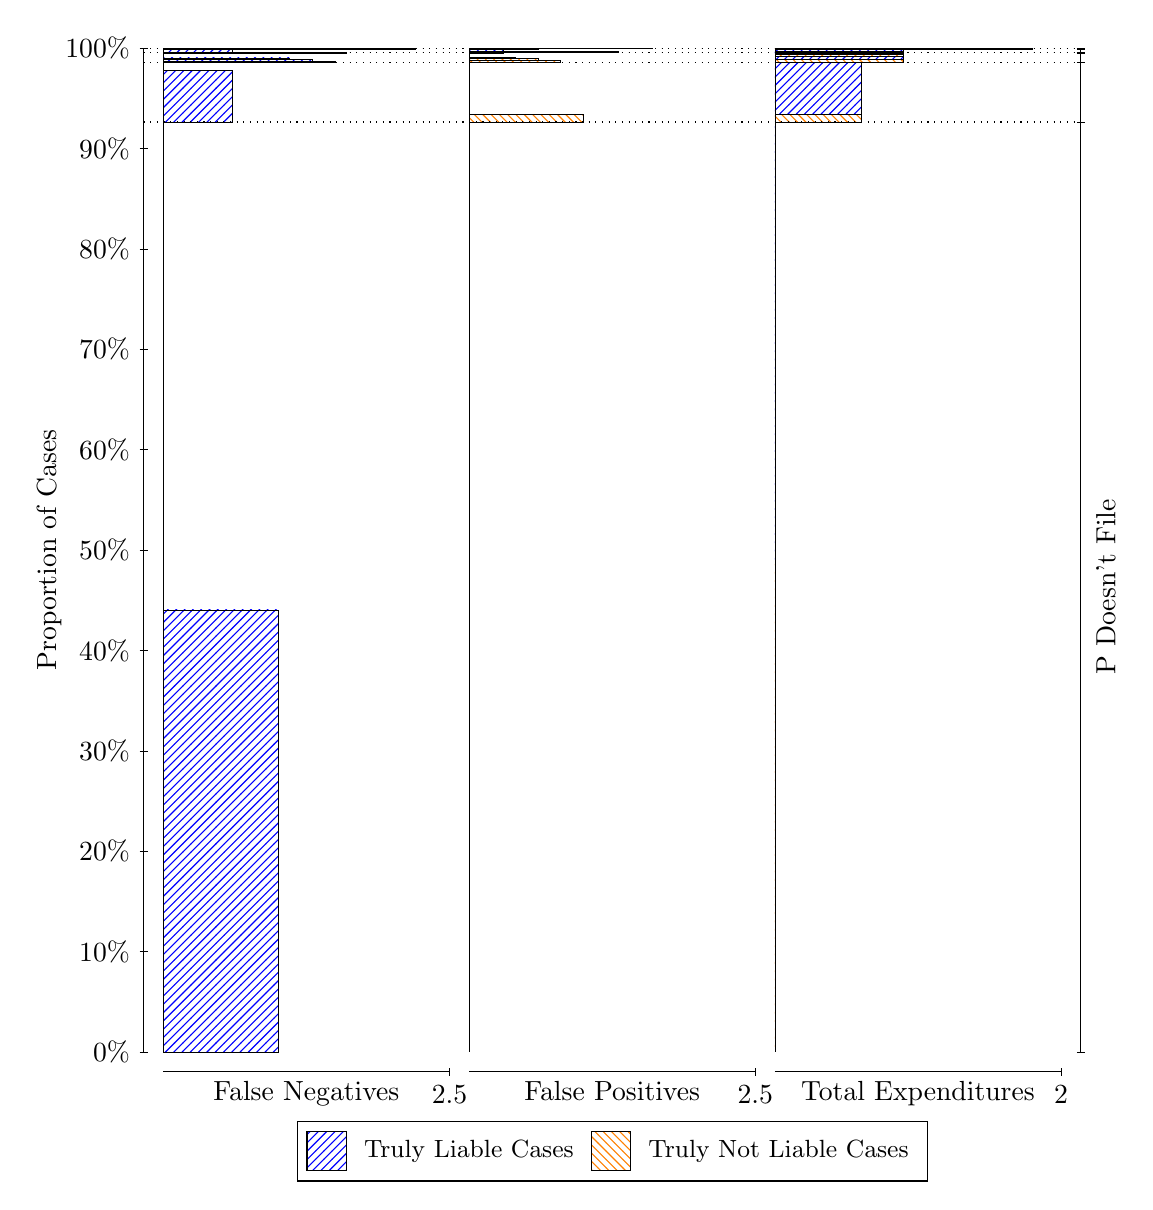
\begin{tikzpicture}
\draw[black, very thin] (1.5,1.75) -- (1.5,14.5);
\node[rotate=90, text=black, anchor=center] at (0.3, 8.125) {Proportion of Cases};
\draw[black, very thin] (1.45,1.75) -- (1.55,1.75);
\node[text=black, anchor=east] at (1.45, 1.75) {0\%};
\draw[black, very thin] (1.45,3.025) -- (1.55,3.025);
\node[text=black, anchor=east] at (1.45, 3.025) {10\%};
\draw[black, very thin] (1.45,4.3) -- (1.55,4.3);
\node[text=black, anchor=east] at (1.45, 4.3) {20\%};
\draw[black, very thin] (1.45,5.575) -- (1.55,5.575);
\node[text=black, anchor=east] at (1.45, 5.575) {30\%};
\draw[black, very thin] (1.45,6.85) -- (1.55,6.85);
\node[text=black, anchor=east] at (1.45, 6.85) {40\%};
\draw[black, very thin] (1.45,8.125) -- (1.55,8.125);
\node[text=black, anchor=east] at (1.45, 8.125) {50\%};
\draw[black, very thin] (1.45,9.4) -- (1.55,9.4);
\node[text=black, anchor=east] at (1.45, 9.4) {60\%};
\draw[black, very thin] (1.45,10.675) -- (1.55,10.675);
\node[text=black, anchor=east] at (1.45, 10.675) {70\%};
\draw[black, very thin] (1.45,11.95) -- (1.55,11.95);
\node[text=black, anchor=east] at (1.45, 11.95) {80\%};
\draw[black, very thin] (1.45,13.225) -- (1.55,13.225);
\node[text=black, anchor=east] at (1.45, 13.225) {90\%};
\draw[black, very thin] (1.45,14.5) -- (1.55,14.5);
\node[text=black, anchor=east] at (1.45, 14.5) {100\%};

\draw[black, very thin] (13.4,1.75) -- (13.4,14.5);
\draw[black, very thin] (13.35,1.75) -- (13.45,1.75);
\node[anchor=west] at (13.35, 1.75) {};
\draw[black, very thin] (13.35,13.56) -- (13.45,13.56);
\node[anchor=west] at (13.35, 13.56) {};
\draw[black, very thin] (13.35,14.314) -- (13.45,14.314);
\node[anchor=west] at (13.35, 14.314) {};
\draw[black, very thin] (13.35,14.438) -- (13.45,14.438);
\node[anchor=west] at (13.35, 14.438) {};
\draw[black, very thin] (13.35,14.447) -- (13.45,14.447);
\node[anchor=west] at (13.35, 14.447) {};
\draw[black, very thin] (13.35,14.49) -- (13.45,14.49);
\node[anchor=west] at (13.35, 14.49) {};
\draw[black, very thin] (13.35,14.494) -- (13.45,14.494);
\node[anchor=west] at (13.35, 14.494) {};
\draw[black, very thin] (13.35,14.5) -- (13.45,14.5);
\node[anchor=west] at (13.35, 14.5) {};

\draw[black, very thin, pattern color=blue, pattern=north east lines] (1.75,1.75) rectangle (3.2033,7.3653);
\draw[black, very thin, pattern color=orange, pattern=north west lines] (1.75,7.3653) rectangle (1.75,13.56);
\draw[black, very thin, pattern color=blue, pattern=north east lines] (1.75,13.56) rectangle (2.622,14.215);
\draw[black, very thin, pattern color=orange, pattern=north west lines] (1.75,14.215) rectangle (1.75,14.314);
\draw[black, very thin, pattern color=blue, pattern=north east lines] (1.75,14.314) rectangle (3.93,14.331);
\draw[black, very thin, pattern color=blue, pattern=north east lines] (1.75,14.331) rectangle (3.6393,14.353);
\draw[black, very thin, pattern color=blue, pattern=north east lines] (1.75,14.353) rectangle (3.3487,14.375);
\draw[black, very thin, pattern color=orange, pattern=north west lines] (1.75,14.375) rectangle (1.75,14.438);
\draw[black, very thin, pattern color=blue, pattern=north east lines] (1.75,14.438) rectangle (4.0753,14.443);
\draw[black, very thin, pattern color=orange, pattern=north west lines] (1.75,14.443) rectangle (1.75,14.447);
\draw[black, very thin, pattern color=blue, pattern=north east lines] (1.75,14.447) rectangle (2.622,14.48);
\draw[black, very thin, pattern color=orange, pattern=north west lines] (1.75,14.48) rectangle (1.75,14.49);
\draw[black, very thin, pattern color=blue, pattern=north east lines] (1.75,14.49) rectangle (4.9473,14.492);
\draw[black, very thin, pattern color=orange, pattern=north west lines] (1.75,14.492) rectangle (1.75,14.494);
\draw[black, very thin, pattern color=blue, pattern=north east lines] (1.75,14.494) rectangle (3.494,14.498);
\draw[black, very thin, pattern color=orange, pattern=north west lines] (1.75,14.498) rectangle (1.75,14.5);
\draw[black, very thin, pattern color=orange, pattern=north west lines] (5.6333,1.75) rectangle (5.6333,7.9449);
\draw[black, very thin, pattern color=blue, pattern=north east lines] (5.6333,7.9449) rectangle (5.6333,13.56);
\draw[black, very thin, pattern color=orange, pattern=north west lines] (5.6333,13.56) rectangle (7.0867,13.659);
\draw[black, very thin, pattern color=blue, pattern=north east lines] (5.6333,13.659) rectangle (5.6333,14.314);
\draw[black, very thin, pattern color=orange, pattern=north west lines] (5.6333,14.314) rectangle (6.796,14.343);
\draw[black, very thin, pattern color=orange, pattern=north west lines] (5.6333,14.343) rectangle (6.5053,14.364);
\draw[black, very thin, pattern color=orange, pattern=north west lines] (5.6333,14.364) rectangle (6.2147,14.377);
\draw[black, very thin, pattern color=blue, pattern=north east lines] (5.6333,14.377) rectangle (5.6333,14.438);
\draw[black, very thin, pattern color=orange, pattern=north west lines] (5.6333,14.438) rectangle (6.0693,14.443);
\draw[black, very thin, pattern color=blue, pattern=north east lines] (5.6333,14.443) rectangle (5.6333,14.447);
\draw[black, very thin, pattern color=orange, pattern=north west lines] (5.6333,14.447) rectangle (7.5227,14.457);
\draw[black, very thin, pattern color=blue, pattern=north east lines] (5.6333,14.457) rectangle (6.0693,14.49);
\draw[black, very thin, pattern color=orange, pattern=north west lines] (5.6333,14.49) rectangle (6.5053,14.492);
\draw[black, very thin, pattern color=blue, pattern=north east lines] (5.6333,14.492) rectangle (5.6333,14.494);
\draw[black, very thin, pattern color=orange, pattern=north west lines] (5.6333,14.494) rectangle (7.9587,14.496);
\draw[black, very thin, pattern color=blue, pattern=north east lines] (5.6333,14.496) rectangle (6.5053,14.5);
\draw[black, very thin, pattern color=orange, pattern=north west lines] (9.5167,1.75) rectangle (9.5167,7.9449);
\draw[black, very thin, pattern color=blue, pattern=north east lines] (9.5167,7.9449) rectangle (9.5167,13.56);
\draw[black, very thin, pattern color=orange, pattern=north west lines] (9.5167,13.56) rectangle (10.607,13.659);
\draw[black, very thin, pattern color=blue, pattern=north east lines] (9.5167,13.659) rectangle (10.607,14.314);
\draw[black, very thin, pattern color=orange, pattern=north west lines] (9.5167,14.314) rectangle (11.152,14.357);
\draw[black, very thin, pattern color=blue, pattern=north east lines] (9.5167,14.357) rectangle (11.152,14.395);
\draw[black, very thin, pattern color=orange, pattern=north west lines] (9.5167,14.395) rectangle (11.152,14.416);
\draw[black, very thin, pattern color=blue, pattern=north east lines] (9.5167,14.416) rectangle (11.152,14.438);
\draw[black, very thin, pattern color=orange, pattern=north west lines] (9.5167,14.438) rectangle (11.152,14.443);
\draw[black, very thin, pattern color=blue, pattern=north east lines] (9.5167,14.443) rectangle (11.152,14.447);
\draw[black, very thin, pattern color=orange, pattern=north west lines] (9.5167,14.447) rectangle (11.152,14.457);
\draw[black, very thin, pattern color=blue, pattern=north east lines] (9.5167,14.457) rectangle (11.152,14.49);
\draw[black, very thin, pattern color=orange, pattern=north west lines] (9.5167,14.49) rectangle (12.787,14.492);
\draw[black, very thin, pattern color=blue, pattern=north east lines] (9.5167,14.492) rectangle (12.787,14.494);
\draw[black, very thin, pattern color=orange, pattern=north west lines] (9.5167,14.494) rectangle (12.787,14.496);
\draw[black, very thin, pattern color=blue, pattern=north east lines] (9.5167,14.496) rectangle (12.787,14.5);
\draw[black, dotted] (1.5,13.56) -- (13.4,13.56);
\draw[black, dotted] (1.5,14.314) -- (13.4,14.314);
\draw[black, dotted] (1.5,14.438) -- (13.4,14.438);
\draw[black, dotted] (1.5,14.447) -- (13.4,14.447);
\draw[black, dotted] (1.5,14.49) -- (13.4,14.49);
\draw[black, dotted] (1.5,14.494) -- (13.4,14.494);
\draw[black, very thin] (1.75,1.5) -- (5.3833,1.5);
\node[text=black, anchor=north] at (3.5667, 1.5) {False Negatives};
\draw[black, very thin] (5.3833,1.45) -- (5.3833,1.55);
\node[text=black, anchor=north] at (5.3833, 1.45) {2.5};

\draw[black, very thin] (5.6333,1.5) -- (9.2667,1.5);
\node[text=black, anchor=north] at (7.45, 1.5) {False Positives};
\draw[black, very thin] (9.2667,1.45) -- (9.2667,1.55);
\node[text=black, anchor=north] at (9.2667, 1.45) {2.5};

\draw[black, very thin] (9.5167,1.5) -- (13.15,1.5);
\node[text=black, anchor=north] at (11.333, 1.5) {Total Expenditures};
\draw[black, very thin] (13.15,1.45) -- (13.15,1.55);
\node[text=black, anchor=north] at (13.15, 1.45) {2};

\node[text=black, centered, rotate=90] at (13.72, 7.6551) {P Doesn't File};







\draw (7.449999999999999,1.5) node[draw=none] (baseCoordinate) {};
\begin{scope}[align=center]
        \matrix[scale=0.5, draw=black, below=0.5cm of baseCoordinate, nodes={draw}, column sep=0.1cm]{
            \node[rectangle, draw, minimum width=0.5cm, minimum height=0.5cm, pattern color=blue, pattern=north east lines] {}; &
            \node[draw=none, font=\small, text=black] (B) {Truly Liable Cases}; &
            \node[rectangle, draw, minimum width=0.5cm, minimum height=0.5cm, pattern color=orange, pattern=north west lines] {}; &
            \node[draw=none, font=\small, text=black] (B) {Truly Not Liable Cases}; \\
            };
\end{scope}

\end{tikzpicture}
\end{document}